\documentclass[10pt]{book}

\usepackage{cdtBook}
\usepackage{requerimientos}

\title{Sistema de Control Radiológico V2.0\\ Etapa I}
\subtitle{\bigskip Propuesta de desarrollo}

%\title{Propuesta Detallada}
%BESP
%\subtitle{Subsistema Banco de Imágenes\\Sistema de Información y Documentación Ambiental}
\author{Coordinación de Desarrollo Tecnológico}
%\organization{Escuela Superior de Cómputo, IPN}
%\date{15 de Junio de 2012}

\newcommand{\nombreProyecto}{Uroboros }
\newcommand{\empresa}{Umbrella }
\newcommand{\cliente}{AlgunWey}

\proyecto[SCOR]{Sistema de Control Radiológico V2.0}
\etapaProy{Inicial}
\usoProy{Externo}

\documento[D--PR]{Propuesta de Desarrollo}
\docVersion{1.0}
%\docFecha{}

%\docRefs{
%	\DRitem{Anexo Técnico}{Anexo Técnico del convenio de colaboración ESCOM-SMA.}
%}

\elaboro[Analista IPN]{José Jaime López Rabadán}
\superviso[Jefe de UPIS de ESCOM]{Ulises Vélez Saldaña}
\aprobo[Responsable del proyecto]{Fernando Ramirez Perez}

 
\begin{document}


\pagestyle{empty}
\ThisURCornerWallPaper{0.4}{images/logos.png}
\maketitle
%\makeDocInfo[9cm]
\frontmatter
\tableofcontents
\mainmatter
\pagestyle{fancy}

% \ThisURCornerWallPaper{0.5}{images/logos2.png}
% \maketitle
% \tableofcontents

%=========================================================
\chapter{Introducción} 

\section{Presentación}

	El presente documento contiene la Propuesta de Desarrollo para el sistema \nombreProyecto      por parte de  \empresa.
	
	La propuesta inicia con la presentación del resultado del análisis realizado y la descripción de los problemas detectados y las necesidades externadas por \cliente.

\section{Antecedentes} 

\Instrucciones{Resumen del proyecto: nombre, partes involucradas, objetivo, alcance, sede, administración, gobierno, fechas de entrega, status actual}

	La presente propuesta es el resultado de un estudio realizado por analistas de \empresa a petición de \cliente.
	
	El objeto de dicho análisis es la revisión del proceso y sistemas existentes para registrar los periodos vacacionales, dias feriados y permisos de faltas de los empleados, que en conjunto, de ahora en adelante seran referidos como faltas. 
	
%TODO: Esta mierda debe de ir? 
%\section{Confidencialidad

%	La presente propuesta se elaboró con base en entrevistas realizadas con la CNSNS y el personal del IPN asignado a este proyecto. La información contenida en este documento es una estimación inicial sujeta a negociación y está dirigida a las personas descritas al final de este documento. Se exige que la información contenida en esta propuesta no sea compartida a terceros, en especial a otros proveedores participantes en el concurso del proyecto en cuestión, sin la autorización previa del IPN mediante el contacto provisto al final del documento.


%=========================================================
\chapter{Diagnóstico} 

	Este capítulo presenta la problemática detectada y ofrece un conjunto de posibles alternativas de solución enfatizando la correspondiente a esta propuesta junto con sus ventajas y desventajas.
	
%---------------------------------------------------------
\section{Situación actual}

	Actualmente \cliente lleva a cabo el control de faltas de manera anacronica utilizando hojas de calculo en excel.
	
\subsection{Proceso de control de faltas.}

	La figura~\ref{fig:procesoLic} muestra el proceso para llevar el control de faltas.

\begin{figure}[htbp!]
	\begin{center}
		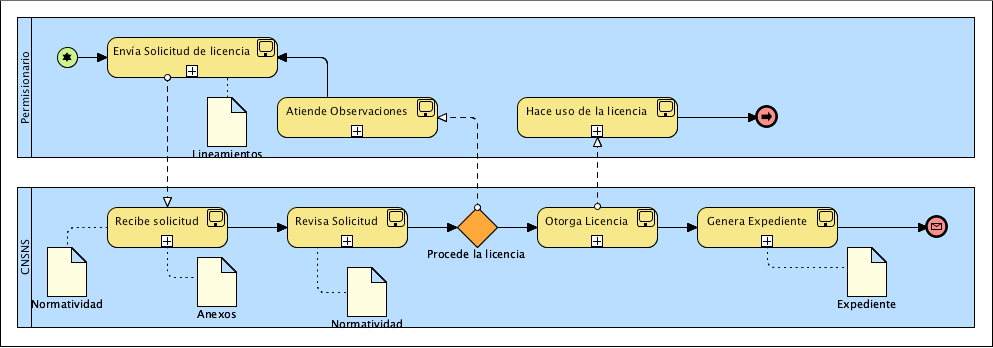
\includegraphics[width=\textwidth]{images/procesoLic}
		\caption{Proceso de control de faltas.}
		\label{fig:procesoLic}
	\end{center}
\end{figure}


%---------------------------------------------------------
\section{Problemas Detectados}
	
	Con base en la revisión del proceso anterior y el sistema semiautomatizado existente, se recopilaron las impresiones y comentarios de los actores del proceso. Los problemas detectados se resumen a continuación:
	
	\begin{itemize}
		\item Plataforma inadecuada. Debido a que la informacion esta en archivos de excel, el compartirla implica hacer copias que no necesariamente tendran la informacion actualizada cuando se consulten.
		\item Bajo desempeño. Ya que no se cuenta con un sistema ni con un equipo dedicado a este proceso.
		\item Falta de Históricos. El sistema solo contempla el registro, por lo que cualquier consulta historica resulta extremadamente tediosa, al punto de ser imposible para fines practicos.
		\item Duplicidad de trabajo. Debido a que el trabajo es manual sobre hojas de excel, no esta diseñado para ser colaborativo y existe el riesgo de duplicidad de informacion.
		\item Poca visibilidad del proceso. Es difícil saber las estadisticas de asistencia de los empleados.
		\item No hay información para la alta gerencia. Los directivos no tienen una vista del sistema que les permita conocer las asistencias y faltas del personal.
	\end{itemize}

%---------------------------------------------------------
\section{Identificación de Causas}

Derivado de la problemática anterior se realizó una estimación de las posibles acudas:

\begin{itemize}	
	\item Plataforma inadecuada. No es un sistema colaborativo, solo quien registra la informacion puede consultarla de manera facil, cuando dicha informacion es actual.
	\item Crecimiento inesperado. La forma como se lleva a cabo el proceso conlleva el problema de que al crecer \cliente en cuanto a numero de personal, se hace cada vez mas inviable tener control.
	\item El Sistema actual no considera que se deben generar informes y tomar desiciones por parte de los diferentes niveles jerarquicos.
\end{itemize}

%---------------------------------------------------------
\section{Estimación de Consecuencias}

\begin{itemize}	
	\item Incumplimiento en los tiempos. La dificultad para explotar los archivos de excel implica que el realizar informes o reportes pueda tomar mas tiempo del que se estima.
	\item Falta de conocimiento de las estadisticas de asistencias. El obtener informacion global de la asistencia de un empleado es muy dificil debido a lo dispersa de la informacion, ademas de que depende en gran medida de los criterios del responsable del registro, con lo que no es facil que reciba ayuda o que alguien tome esa responsabilidad.
	\item Caos en la información. Con un alto volumen de información, se perderá el control de lo que se contiene hojas de excel.
\end{itemize}


%---------------------------------------------------------
\section{Conclusión del análisis}
	
	Una de las principales necesidades actualmente es facilitar el registro de las faltas, de manera que el usuario solo tenga que ingresar los datos y el sistema se encargue la informacion que el usuario requiere en forma de reportes .
	
	El sistema \nombreProyecto debe contemplar la gerencia y toma de decisiones a traves de facilidades de reporteria que faciliten la consulta de la informacion a los distintos niveles jerarquicos.
	
	Con base en lo anterior se considera que el desarrollo pueda llevar un proceso con las siguiente setapas:
	
\begin{itemize}
	\item Análisis y definición del proceso de registro de faltas.
	\item Migración de información.
	\item Implementación del nuevo proceso y puesta en marcha de los nuevos sistemas.
\end{itemize}

%=========================================================
\chapter{Alcance de la Propuesta}

	La siguiente propuesta plantea la primera etapa del proyecto considerando cinco meses como tiempo disponible.

%---------------------------------------------------------
\section{Objetivo General}

	Elaboración de análisis de requerimientos y prototipo conceptual de \nombreProyecto.
%---------------------------------------------------------
\section{Objetivos Específicos}

\begin{itemize}
	\item Análisis del proceso de registro y control de faltas.
	\item Elaboración del prototipo conceptual.
	\item Diseño de las vistas y reportes requeridos por \cliente.
\end{itemize}

%---------------------------------------------------------
%\section{Requerimientos}
%
%
%\subsection{Modelo de Despliegue}
%
%\subsubsection{Hardware}
%
%\subsubsection{Software}

%\subsection{Requerimientos funcionales}
	
	
%=========================================================
\chapter{Metodología}


%---------------------------------------------------------
\section{Proceso}

	La elaboración del análisis y construcción del prototipo conceptual se llevará mediante el siguiente proceso:
	
	
\begin{enumerate}
	\item {\bf Toma de Requerimientos.} Mediante mesas de trabajo, entrevistas personales, elaboración de encuestas, inspección de la operación y análisis documental de evidencias, normas y reglamentos aplicables se integra el expediente base para la realización del análisis.
	\item {\bf Organización y análisis.} Se aplica un proceso de organización y análisis de la problemática que permitirá determinar: el nuevo proceso a seguir y la funcionalidad que deberá presentar el sistema. Esto con base en un enfoque de aprovechamiento de las distintas áreas de oportunidad identificadas y la aplicación de nuevas tecnologías de información en la operación.
	\item {\bf Verificación y retroalimentación del diseño.} Mediante mesas de trabajo, entrevistas y retroalimentación con la CNSNS se presentan los resultados del análisis a fin de verificar la viabilidad y alcance de su aplicación con base en los recursos y capacidades del personal, tecnología e infraestructura de la CNSNS.
	\item {\bf Especificación formal del sistema.} Se genera un documento detallado y conciso con todos los detalles que deberá tener el nuevo proceso y el SCOR V2.0 para su aprobación.  
	\item {\bf Aprobación de acuerdos.} Una vez establecidos los acuerdos, se presenta la especificación para su lectura, análisis y aprobación por ambas partes.
	\item {\bf Presentación del Prototipo Conceptual.} Se construye y presenta una maqueta del sistema ({\em Prototipo Conceptual}) que permita evaluar la interacción del sistema con los usuarios.
\end{enumerate}

%---------------------------------------------------------
\section{Especificación Formal}

	Consiste en un documento que contiene la siguiente información:
	
\begin{itemize}
	\item {\bf Introducción.} Contiene la presentación del documento, contenido, organización, etc.
	\item {\bf Modelo del negocio.} Presenta las consideraciones propias de la operación y la organización que gobiernan al sistema, entre ellas: Glosario de términos, normatividad aplicable, procesos, roles, modelo estructural del negocio y reglas de operación.
	\item {\bf Modelo de despliegue.} Especifica las características de Software, Hardware y servicios de comunicación necesarios para que opere el sistema y la arquitectura del sistema.
	\item {\bf Modelo del Comportamiento.} Describe mediante casos de uso toda la funcionalidad paso a paso del sistema especificando, el propósito de cada funcionalidad del sistema, las operaciones involucradas, los efectos colaterales de cada operación, los prerequicitos, el control de acceso a las operaciones y las responsabilidades, tanto de los usuarios como del sistema, durante la operación.
	\item {\bf Modelo de interacción.} Especifica, a manera de manual de usuario todas las interfaces del sistema y la forma en que deben usarse, incluyendo una lista con todos los mensajes, correos, avisos y notificaciones que pueda generar el sistema.
\end{itemize}


%---------------------------------------------------------
\section{Ambiente de Pruebas}

	El ambiente de pruebas consiste en una carpeta con archivos en formato HTML, que contiene el Prototipo Conceptual y se puede utilizar para verificar el comportamiento que tendrá el sistema.

%---------------------------------------------------------
\section{Entregables}
	
	Al término del proyecto los productos que se entregarán son:
	
\begin{description}
	\item [Entregable I.] Expediente de análisis. Carpeta con toda la documentación recabada, informes y evidencias de las entrevistas y mesas de trabajo
	\item [Entregable II.] Diagnóstico inicial. Contiene el análisis de la problemática, las oportunidades de mejora de procesos y las tecnologías que se pueden aprovechar en la operación.
	\item [Entregable III.] Especificación Formal. Que contiene la especificación del SCOR V2.0.
	\item [Entregable IV.] Prototipo Conceptual. Construcción y programación de la navegación y mensajes de las pantallas del SCOR V2.0.
\end{description}


\section{Tiempos y Costos del proyecto}

	En esta sección se describen los tiempos y los montos correspondientes a cada entrega del sistema. Los  tiempos se consideran a partir de la firma del convenio.\\

\begin{tabular}{|l | l | r|}
	\hline
	{\bf Entregable}& {\bf Fecha} &{\bf Monto}  \\
	\hline
	I & Primeras dos semanas  & \$ 500,000.00+IVA\\
	\hline
	II & Mes y medio & \$ 700,000.00+IVA\\
	\hline
	III & Tercer mes & \$ 700,000.00+IVA\\
	\hline
	IV & Quinto mes & \$ 600,000.00+IVA\\
	\hline
	\hline
	 & Total & \$ 2,500,000.00+IVA\\
	\hline
\end{tabular}

\clossing

\end{document}